\documentclass[a4paper,11pt]{article}

% Kodovani (cestiny) v dokumentu: utf-8
%\usepackage[cp1250]{inputenc}	% Omezena stredoevropska kodova stranka, pouze MSW.
\usepackage[utf8]{inputenc}	% Doporucujeme pouzivat UTF-8 (unicode).

\usepackage[margin=2cm]{geometry}
\newtoks\jmenopraktika \newtoks\jmeno \newtoks\datum
\newtoks\obor \newtoks\skupina \newtoks\rocnik \newtoks\semestr
\newtoks\cisloulohy \newtoks\jmenoulohy
\newtoks\tlak \newtoks\teplota \newtoks\vlhkost

\jmenopraktika={Fyzikální praktikum 3}
\jmeno={Lukáš Lejdar}
\datum={26. února 2025}
\obor={F}
\skupina={Út 14:00}

\cisloulohy={7}
\jmenoulohy={Optická emisní spektra atomů a molekul}

\tlak={101{,}35}
\teplota={21,1}
\vlhkost={47,7}


%%%%%%%%%%% Uzitecne balicky:
\usepackage[czech]{babel}

\usepackage{graphicx}
\usepackage{amsmath}
\usepackage{xspace}
\usepackage{url}
\usepackage{indentfirst}
\usepackage{wrapfig}
\usepackage{xcolor}
\usepackage{subfig}
\usepackage{subcaption}
\usepackage{enumitem}
\usepackage{tikzsymbols}
\usepackage{newfloat}
\usepackage{multicol}
\usepackage{float}

\DeclareFloatingEnvironment[fileext=lof]{graph}
\captionsetup[graph]{labelformat=simple, labelsep=colon, name=Graf}

%%%%%% Zamezeni parchantu:
\widowpenalty 10000 \clubpenalty 10000 \displaywidowpenalty 10000
%%%%%% Parametry pro moznost vsazeni vetsiho poctu obrazku na stranku
\setcounter{topnumber}{3}	  % max. pocet floatu nahore (specifikace t)
\setcounter{bottomnumber}{3}	  % max. pocet floatu dole (specifikace b)
\setcounter{totalnumber}{6}	  % max. pocet floatu na strance celkem
\renewcommand\topfraction{0.9}	  % max podil stranky pro floaty nahore
\renewcommand\bottomfraction{0.9} % max podil stranky pro floaty dole
\renewcommand\textfraction{0.1}	  % min podil stranky, ktery musi obsahovat text
\intextsep=8mm \textfloatsep=8mm  %\intextsep pro ulozeni [h] floatu a \textfloatsep pro [b] or [t]

% Tecky za cisly sekci:
\renewcommand{\thesection}{\arabic{section}.}
\renewcommand{\thesubsection}{\thesection\arabic{subsection}.}
% Jednopismenna mezera mezi cislem a nazvem kapitoly:
\makeatletter \def\@seccntformat#1{\csname the#1\endcsname\hspace{1ex}} \makeatother
%
\newcommand{\vsn}[4]{\ensuremath{#1 =} #2(#3)\,#4}
\newcommand{\vrn}[6]{\ensuremath{#1 =} (#2 $\pm$ #3)\,#4 ($p=$ #5\,\%, $\nu=$ #6)}

\newcommand*\circled[1]{\tikz[baseline=(char.base)]{
		\node[shape=circle,draw,inner sep=1pt] (char) {#1};}}

%%%%%%%%%%%%%%%%%%%%%%%%%%%%%%%%%%%%%%%%%%%%%%%%%%%%%%%%%%%%%%%%%%%%%%%%%%%%%%%
% Zacatek dokumentu
%%%%%%%%%%%%%%%%%%%%%%%%%%%%%%%%%%%%%%%%%%%%%%%%%%%%%%%%%%%%%%%%%%%%%%%%%%%%%%%

\begin{document}

\thispagestyle{empty}

{
\begin{center}
\sf 
{\Large Ústav fyziky a technologií plazmatu Přírodovědecké fakulty Masarykovy univerzity} \\
\bigskip
{\huge \bfseries FYZIKÁLNÍ PRAKTIKUM} \\
\bigskip
{\Large \the\jmenopraktika}
\end{center}

\bigskip

\sf
\noindent
\setlength{\arrayrulewidth}{1pt}
\begin{tabular*}{\textwidth}{@{\extracolsep{\fill}} l l}
\large {\bfseries Zpracoval:}  \the\jmeno & \large  {\bfseries Naměřeno:} \the\datum\\[2mm]
\large  {\bfseries Obor:} \the\obor  \hspace{40mm}  {\bfseries Skupina:} \the\skupina %
&\large {\bfseries Testováno:}\\
\\
\hline
\end{tabular*}
}

\bigskip

{
\sf
\noindent \begin{tabular}{p{4cm} p{0.6\textwidth}}
\Large  Úloha č. {\bfseries \the\cisloulohy:} \par
\smallskip
$T=\the\teplota$~$^\circ$C \par
$p=\the\tlak$~kPa \par
$\varphi=\the\vlhkost$~\%
&\Large \bfseries \the\jmenoulohy  \\[2mm]
\end{tabular}
}

\vskip1cm

\section{Úvod}

Cílem úlohy je identifikovat spektrální čáry par železa v obloukovém výboji a molekulové spektrum radikálů OH, měřené v nízkoteplotním plazmatu. Z obou spekter potom zjistím příslušnou teplotu plazmatu ze sklonu pyrometrické přímky.
 
\section{Teorie}

\subsection{Intenzita spektrálních čar}

Při přechodu elektronu z m-té hladiny o energii \( E_m \) na nižší s energií \( E_n \) se vyzáří světlo, které pozorujeme jako spektrální čáru o vlnové délce \( \lambda_{mn} \) a relativní intenzitě

\begin{equation}
    I_{mn} =  \frac{A_{mn}g_m}{\lambda_{mn}} \exp \left( -\frac{E_m}{kT} \right),
\end{equation}

\noindent
kde $ A_{mn} $  je pravděpodobnost přechodu z m-té hladiny na n-tou a $ g_m $  je statistická váha horního energetického stavu. Experimentálně jsou přímo měřitelné intenzity spektrálních čar a ke každé známe i součin $ A_{mn} g_m $ a excitační energie $ E_m $. Úpravou vztahu (1) dostávám

\begin{equation}
\ln \left( \frac{I_{mn}\lambda_{mn}}{A_{mn}g_m} \right) = \left( - \frac{E_m}{kT} \right) = f(E_m).
\end{equation}

Graf závislosti $ f(E_m) $ je známý jako pyrometrická přímka se sklonem $ - \frac{1}{kT} $.

\subsection{Intenzita rotační čáry}

Rotační energie molekuly je na rozdíl od té translační kvantovaná. Můžeme tedy pozorovat i spektrální čáry způsobené změnou stavu rotace molekuly a pro její intenzitu platí vztah

\begin{equation}
I_{n''v''J''}^{n'v'J'} = C_{n''v''J''}^{n'v'J'} \bar{\nu}^{4} S_{J'J''}e^{-\frac{B_{v'} N' (N' + 1) hc}{kT}}
\end{equation}

\noindent
$ B_{v'} $  je rotační konstanta pro horní vibrační stav, $ N' $  je rotační kvantové číslo horního stavu, $ \bar{\nu}^{4} = \lambda^{-4} $ je vlnočet rotační čáry, $ S_{J'J''} $ je Hönl-Londonův intenzitní faktor a $ J' $ je kvantové číslo pro celkový moment hybnosti. V případě dat měřených v praktiku platí $ N' = J' - \frac{1}{2} $. Rovnici (3) můžeme opět upravit na pyrometrický tvar

\begin{equation}
\ln \frac{I_{n''v''J''}^{n'v'J'}}{\bar{\nu}^{4} S_{J'J''}} = -\frac{B_{v'} hc}{kT} N' (N' + 1)  + konst. = f(N' (N' + 1))
\end{equation}


\newpage

\section{Výsledky měření}

\subsection{Atomové spektrum par železa}

Spektrální závislost z grafu 1 jsem dostal už naměřenou a data jsem jen zpracovával. Soubor jsem otevřel v programu Span 1.7 a označil vybrané spektrální čáry pro vlnové délky podle tabulky 1, kde ve 4. sloupci jsou i programem odečtené intenzity

\begin{figure}[htpb]
    \centering
    % GNUPLOT: LaTeX picture with Postscript
\begingroup
  \makeatletter
  \providecommand\color[2][]{%
    \GenericError{(gnuplot) \space\space\space\@spaces}{%
      Package color not loaded in conjunction with
      terminal option `colourtext'%
    }{See the gnuplot documentation for explanation.%
    }{Either use 'blacktext' in gnuplot or load the package
      color.sty in LaTeX.}%
    \renewcommand\color[2][]{}%
  }%
  \providecommand\includegraphics[2][]{%
    \GenericError{(gnuplot) \space\space\space\@spaces}{%
      Package graphicx or graphics not loaded%
    }{See the gnuplot documentation for explanation.%
    }{The gnuplot epslatex terminal needs graphicx.sty or graphics.sty.}%
    \renewcommand\includegraphics[2][]{}%
  }%
  \providecommand\rotatebox[2]{#2}%
  \@ifundefined{ifGPcolor}{%
    \newif\ifGPcolor
    \GPcolorfalse
  }{}%
  \@ifundefined{ifGPblacktext}{%
    \newif\ifGPblacktext
    \GPblacktexttrue
  }{}%
  % define a \g@addto@macro without @ in the name:
  \let\gplgaddtomacro\g@addto@macro
  % define empty templates for all commands taking text:
  \gdef\gplbacktext{}%
  \gdef\gplfronttext{}%
  \makeatother
  \ifGPblacktext
    % no textcolor at all
    \def\colorrgb#1{}%
    \def\colorgray#1{}%
  \else
    % gray or color?
    \ifGPcolor
      \def\colorrgb#1{\color[rgb]{#1}}%
      \def\colorgray#1{\color[gray]{#1}}%
      \expandafter\def\csname LTw\endcsname{\color{white}}%
      \expandafter\def\csname LTb\endcsname{\color{black}}%
      \expandafter\def\csname LTa\endcsname{\color{black}}%
      \expandafter\def\csname LT0\endcsname{\color[rgb]{1,0,0}}%
      \expandafter\def\csname LT1\endcsname{\color[rgb]{0,1,0}}%
      \expandafter\def\csname LT2\endcsname{\color[rgb]{0,0,1}}%
      \expandafter\def\csname LT3\endcsname{\color[rgb]{1,0,1}}%
      \expandafter\def\csname LT4\endcsname{\color[rgb]{0,1,1}}%
      \expandafter\def\csname LT5\endcsname{\color[rgb]{1,1,0}}%
      \expandafter\def\csname LT6\endcsname{\color[rgb]{0,0,0}}%
      \expandafter\def\csname LT7\endcsname{\color[rgb]{1,0.3,0}}%
      \expandafter\def\csname LT8\endcsname{\color[rgb]{0.5,0.5,0.5}}%
    \else
      % gray
      \def\colorrgb#1{\color{black}}%
      \def\colorgray#1{\color[gray]{#1}}%
      \expandafter\def\csname LTw\endcsname{\color{white}}%
      \expandafter\def\csname LTb\endcsname{\color{black}}%
      \expandafter\def\csname LTa\endcsname{\color{black}}%
      \expandafter\def\csname LT0\endcsname{\color{black}}%
      \expandafter\def\csname LT1\endcsname{\color{black}}%
      \expandafter\def\csname LT2\endcsname{\color{black}}%
      \expandafter\def\csname LT3\endcsname{\color{black}}%
      \expandafter\def\csname LT4\endcsname{\color{black}}%
      \expandafter\def\csname LT5\endcsname{\color{black}}%
      \expandafter\def\csname LT6\endcsname{\color{black}}%
      \expandafter\def\csname LT7\endcsname{\color{black}}%
      \expandafter\def\csname LT8\endcsname{\color{black}}%
    \fi
  \fi
    \setlength{\unitlength}{0.0500bp}%
    \ifx\gptboxheight\undefined%
      \newlength{\gptboxheight}%
      \newlength{\gptboxwidth}%
      \newsavebox{\gptboxtext}%
    \fi%
    \setlength{\fboxrule}{0.5pt}%
    \setlength{\fboxsep}{1pt}%
    \definecolor{tbcol}{rgb}{1,1,1}%
\begin{picture}(9504.00,3744.00)%
    \gplgaddtomacro\gplbacktext{%
      \csname LTb\endcsname%%
      \put(1078,112){\makebox(0,0)[r]{\strut{}$0$}}%
      \put(1078,538){\makebox(0,0)[r]{\strut{}$2000$}}%
      \put(1078,965){\makebox(0,0)[r]{\strut{}$4000$}}%
      \put(1078,1391){\makebox(0,0)[r]{\strut{}$6000$}}%
      \put(1078,1818){\makebox(0,0)[r]{\strut{}$8000$}}%
      \put(1078,2244){\makebox(0,0)[r]{\strut{}$10000$}}%
      \put(1078,2670){\makebox(0,0)[r]{\strut{}$12000$}}%
      \put(1078,3097){\makebox(0,0)[r]{\strut{}$14000$}}%
      \put(1078,3523){\makebox(0,0)[r]{\strut{}$16000$}}%
      \put(1920,-680){\rotatebox{90}{\makebox(0,0)[l]{\strut{}429.413}}}%
      \put(2061,-680){\rotatebox{90}{\makebox(0,0)[l]{\strut{}429.924}}}%
      \put(2302,-680){\rotatebox{90}{\makebox(0,0)[l]{\strut{}430.791}}}%
      \put(2501,-680){\rotatebox{90}{\makebox(0,0)[l]{\strut{}431.509}}}%
      \put(2798,-680){\rotatebox{90}{\makebox(0,0)[l]{\strut{}432.576}}}%
      \put(3111,-680){\rotatebox{90}{\makebox(0,0)[l]{\strut{}433.705}}}%
      \put(3547,-680){\rotatebox{90}{\makebox(0,0)[l]{\strut{}435.274}}}%
      \put(4020,-680){\rotatebox{90}{\makebox(0,0)[l]{\strut{}436.977}}}%
      \put(4191,-680){\rotatebox{90}{\makebox(0,0)[l]{\strut{}437.593}}}%
      \put(4403,-680){\rotatebox{90}{\makebox(0,0)[l]{\strut{}438.357}}}%
      \put(4991,-680){\rotatebox{90}{\makebox(0,0)[l]{\strut{}440.475}}}%
      \put(5279,-680){\rotatebox{90}{\makebox(0,0)[l]{\strut{}441.512}}}%
      \put(5617,-680){\rotatebox{90}{\makebox(0,0)[l]{\strut{}442.731}}}%
      \put(6034,-680){\rotatebox{90}{\makebox(0,0)[l]{\strut{}444.234}}}%
      \put(6184,-680){\rotatebox{90}{\makebox(0,0)[l]{\strut{}444.772}}}%
      \put(6500,-680){\rotatebox{90}{\makebox(0,0)[l]{\strut{}445.912}}}%
      \put(6707,-680){\rotatebox{90}{\makebox(0,0)[l]{\strut{}446.655}}}%
      \put(6969,-680){\rotatebox{90}{\makebox(0,0)[l]{\strut{}447.602}}}%
      \put(7140,-680){\rotatebox{90}{\makebox(0,0)[l]{\strut{}448.217}}}%
      \put(7485,-680){\rotatebox{90}{\makebox(0,0)[l]{\strut{}449.457}}}%
      \put(8430,-680){\rotatebox{90}{\makebox(0,0)[l]{\strut{}452.862}}}%
    }%
    \gplgaddtomacro\gplfronttext{%
      \csname LTb\endcsname%%
      \put(209,1817){\rotatebox{-270}{\makebox(0,0){\strut{}I (a.u.)}}}%
      \put(5158,-1098){\makebox(0,0){\strut{}$\lambda$ (nm)}}%
    }%
    \gplbacktext
    \put(0,0){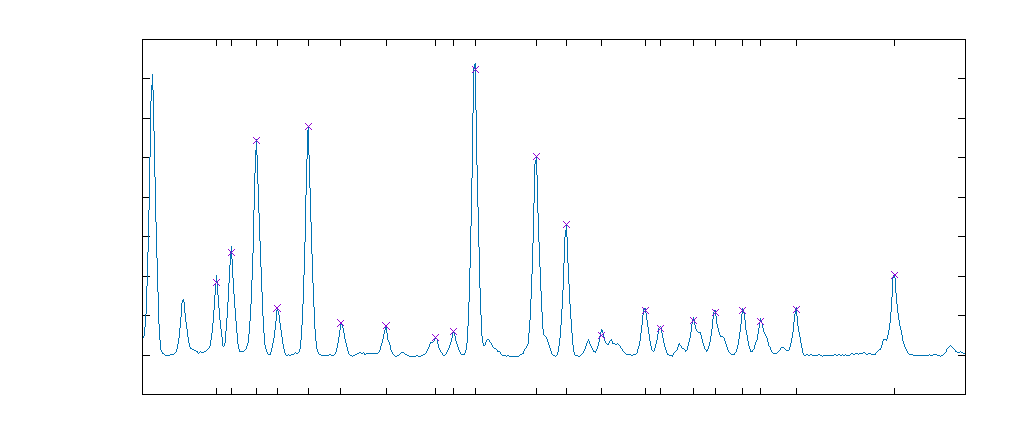
\includegraphics[width={475.20bp},height={187.20bp}]{fe7_data}}%
    \gplfronttext
  \end{picture}%
\endgroup

    \vspace{40pt}
    \captionsetup{type=graph}
    \caption{Naměřená spektrální závislost par železa měřené v obloukovém výboji. Graf je korektovaný podle známých vlnových délek spektrálních čar a šumu pozadí.}
\end{figure}

\vspace{-20pt}

\begin{table}[htpb]
    \begin{minipage}[b]{.65\linewidth}

Z tabulky 1 jsem potom sestrojil graf 2 podle rovnice $ y = f(E_m) $ ze vztahu 2 a z fitu přímkou určil teplotu plazmatu.
\begin{align*}
    a &= -1.94015 \pm 0.1613     \\
    k &= 8.6173303 \cdot 10^{-5} \ eV K^{-1} \\
    T &= 6000 \pm 500 \ K
\end{align*}
\vspace{-30pt}
\begin{figure}[H]
    \centering
    % GNUPLOT: LaTeX picture with Postscript
\begingroup
  \makeatletter
  \providecommand\color[2][]{%
    \GenericError{(gnuplot) \space\space\space\@spaces}{%
      Package color not loaded in conjunction with
      terminal option `colourtext'%
    }{See the gnuplot documentation for explanation.%
    }{Either use 'blacktext' in gnuplot or load the package
      color.sty in LaTeX.}%
    \renewcommand\color[2][]{}%
  }%
  \providecommand\includegraphics[2][]{%
    \GenericError{(gnuplot) \space\space\space\@spaces}{%
      Package graphicx or graphics not loaded%
    }{See the gnuplot documentation for explanation.%
    }{The gnuplot epslatex terminal needs graphicx.sty or graphics.sty.}%
    \renewcommand\includegraphics[2][]{}%
  }%
  \providecommand\rotatebox[2]{#2}%
  \@ifundefined{ifGPcolor}{%
    \newif\ifGPcolor
    \GPcolorfalse
  }{}%
  \@ifundefined{ifGPblacktext}{%
    \newif\ifGPblacktext
    \GPblacktexttrue
  }{}%
  % define a \g@addto@macro without @ in the name:
  \let\gplgaddtomacro\g@addto@macro
  % define empty templates for all commands taking text:
  \gdef\gplbacktext{}%
  \gdef\gplfronttext{}%
  \makeatother
  \ifGPblacktext
    % no textcolor at all
    \def\colorrgb#1{}%
    \def\colorgray#1{}%
  \else
    % gray or color?
    \ifGPcolor
      \def\colorrgb#1{\color[rgb]{#1}}%
      \def\colorgray#1{\color[gray]{#1}}%
      \expandafter\def\csname LTw\endcsname{\color{white}}%
      \expandafter\def\csname LTb\endcsname{\color{black}}%
      \expandafter\def\csname LTa\endcsname{\color{black}}%
      \expandafter\def\csname LT0\endcsname{\color[rgb]{1,0,0}}%
      \expandafter\def\csname LT1\endcsname{\color[rgb]{0,1,0}}%
      \expandafter\def\csname LT2\endcsname{\color[rgb]{0,0,1}}%
      \expandafter\def\csname LT3\endcsname{\color[rgb]{1,0,1}}%
      \expandafter\def\csname LT4\endcsname{\color[rgb]{0,1,1}}%
      \expandafter\def\csname LT5\endcsname{\color[rgb]{1,1,0}}%
      \expandafter\def\csname LT6\endcsname{\color[rgb]{0,0,0}}%
      \expandafter\def\csname LT7\endcsname{\color[rgb]{1,0.3,0}}%
      \expandafter\def\csname LT8\endcsname{\color[rgb]{0.5,0.5,0.5}}%
    \else
      % gray
      \def\colorrgb#1{\color{black}}%
      \def\colorgray#1{\color[gray]{#1}}%
      \expandafter\def\csname LTw\endcsname{\color{white}}%
      \expandafter\def\csname LTb\endcsname{\color{black}}%
      \expandafter\def\csname LTa\endcsname{\color{black}}%
      \expandafter\def\csname LT0\endcsname{\color{black}}%
      \expandafter\def\csname LT1\endcsname{\color{black}}%
      \expandafter\def\csname LT2\endcsname{\color{black}}%
      \expandafter\def\csname LT3\endcsname{\color{black}}%
      \expandafter\def\csname LT4\endcsname{\color{black}}%
      \expandafter\def\csname LT5\endcsname{\color{black}}%
      \expandafter\def\csname LT6\endcsname{\color{black}}%
      \expandafter\def\csname LT7\endcsname{\color{black}}%
      \expandafter\def\csname LT8\endcsname{\color{black}}%
    \fi
  \fi
    \setlength{\unitlength}{0.0500bp}%
    \ifx\gptboxheight\undefined%
      \newlength{\gptboxheight}%
      \newlength{\gptboxwidth}%
      \newsavebox{\gptboxtext}%
    \fi%
    \setlength{\fboxrule}{0.5pt}%
    \setlength{\fboxsep}{1pt}%
    \definecolor{tbcol}{rgb}{1,1,1}%
\begin{picture}(5760.00,2880.00)%
    \gplgaddtomacro\gplbacktext{%
      \csname LTb\endcsname%%
      \put(682,86){\makebox(0,0)[r]{\strut{}$28$}}%
      \put(682,372){\makebox(0,0)[r]{\strut{}$29$}}%
      \put(682,658){\makebox(0,0)[r]{\strut{}$30$}}%
      \put(682,944){\makebox(0,0)[r]{\strut{}$31$}}%
      \put(682,1230){\makebox(0,0)[r]{\strut{}$32$}}%
      \put(682,1515){\makebox(0,0)[r]{\strut{}$33$}}%
      \put(682,1801){\makebox(0,0)[r]{\strut{}$34$}}%
      \put(682,2087){\makebox(0,0)[r]{\strut{}$35$}}%
      \put(682,2373){\makebox(0,0)[r]{\strut{}$36$}}%
      \put(682,2659){\makebox(0,0)[r]{\strut{}$37$}}%
      \put(1228,-134){\makebox(0,0){\strut{}$3$}}%
      \put(1917,-134){\makebox(0,0){\strut{}$3.5$}}%
      \put(2606,-134){\makebox(0,0){\strut{}$4$}}%
      \put(3295,-134){\makebox(0,0){\strut{}$4.5$}}%
      \put(3985,-134){\makebox(0,0){\strut{}$5$}}%
      \put(4674,-134){\makebox(0,0){\strut{}$5.5$}}%
      \put(5363,-134){\makebox(0,0){\strut{}$6$}}%
    }%
    \gplgaddtomacro\gplfronttext{%
      \csname LTb\endcsname%%
      \put(209,1372){\rotatebox{-270}{\makebox(0,0){\strut{}$  \ln \frac{I_{mn} \lambda_{mn} }{ A_{mn}g_m } $}}}%
      \put(3088,-464){\makebox(0,0){\strut{}$E_m$ (eV)}}%
      \csname LTb\endcsname%%
      \put(4376,2486){\makebox(0,0)[r]{\strut{}$ ax + b $}}%
    }%
    \gplbacktext
    \put(0,0){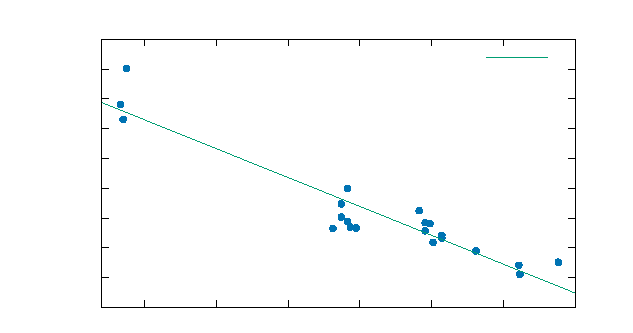
\includegraphics[width={288.00bp},height={144.00bp}]{fe7_pyrometra}}%
    \gplfronttext
  \end{picture}%
\endgroup

    \captionsetup{type=graph}
    \caption{Pyrometrická přímka par železa}
\end{figure}

    \end{minipage} 
    \hfill
    \begin{minipage}[b]{.3\linewidth}
        \centering

\begin{table}[H]
    \vspace{-43pt}
    \small
    \centering
    \begin{tabular}{l l l l}
        $ \lambda_{mn} $ & $ E_m $ & $ A_{mn}g_m $ & I   \\ \hline
        (nm) & (eV) & (s$ ^{-1} $) & (a.u.) \\ \hline\hline
        429.413 & 4.371 & 0.71   &  774 \\
        429.924 & 5.308 & 5.2    & 1166 \\
        430.791 & 4.434 & 5.9    & 2924 \\
        431.509 & 5.070 & 1.5    &  564 \\
        432.576 & 4.473 & 6.1    & 2930 \\
        433.705 & 4.415 & 0.23   &  416 \\
        435.274 & 5.070 & 1.0    &  341 \\
        436.977 & 5.882 & 2.2    &  331 \\
        437.593 & 2.832 & 0.0094 &  284 \\
        438.357 & 4.312 & 7.7    & 3585 \\
        440.475 & 4.371 & 4.4    & 2992 \\
        441.512 & 4.415 & 2.8    & 1637 \\
        442.731 & 2.851 & 0.0099 &  178 \\
        444.234 & 4.988 & 1.1    &  597 \\
        444.772 & 5.009 & 1.1    &  316 \\
        445.912 & 4.955 & 1.0    &  556 \\
        446.655 & 5.606 & 5.3    &  705 \\
        447.602 & 5.614 & 5.4    &  527 \\
        448.217 & 2.875 & 0.0053 &  518 \\
        449.457 & 4.955 & 1.22   &  513 \\
        452.862 & 4.913 & 1.8    & 1476 \\
    \end{tabular}
    \caption{Parametry spektrálních čar}
\end{table}

    \end{minipage} 
\end{table}

\subsection{Spektrum radikálů OH}

Data jsem zase dostal už naměřená a zpracovávání probíhalo podobně jako v předchozím případě. Nejdřív jsem označil spektrální čáry z tabulky 2, které odpovídají rotačním přechodům a pomocí programu Span 1.7 zjistil jejich intenzitu.

\begin{figure}[htpb]
    \centering
    % GNUPLOT: LaTeX picture with Postscript
\begingroup
  \makeatletter
  \providecommand\color[2][]{%
    \GenericError{(gnuplot) \space\space\space\@spaces}{%
      Package color not loaded in conjunction with
      terminal option `colourtext'%
    }{See the gnuplot documentation for explanation.%
    }{Either use 'blacktext' in gnuplot or load the package
      color.sty in LaTeX.}%
    \renewcommand\color[2][]{}%
  }%
  \providecommand\includegraphics[2][]{%
    \GenericError{(gnuplot) \space\space\space\@spaces}{%
      Package graphicx or graphics not loaded%
    }{See the gnuplot documentation for explanation.%
    }{The gnuplot epslatex terminal needs graphicx.sty or graphics.sty.}%
    \renewcommand\includegraphics[2][]{}%
  }%
  \providecommand\rotatebox[2]{#2}%
  \@ifundefined{ifGPcolor}{%
    \newif\ifGPcolor
    \GPcolorfalse
  }{}%
  \@ifundefined{ifGPblacktext}{%
    \newif\ifGPblacktext
    \GPblacktexttrue
  }{}%
  % define a \g@addto@macro without @ in the name:
  \let\gplgaddtomacro\g@addto@macro
  % define empty templates for all commands taking text:
  \gdef\gplbacktext{}%
  \gdef\gplfronttext{}%
  \makeatother
  \ifGPblacktext
    % no textcolor at all
    \def\colorrgb#1{}%
    \def\colorgray#1{}%
  \else
    % gray or color?
    \ifGPcolor
      \def\colorrgb#1{\color[rgb]{#1}}%
      \def\colorgray#1{\color[gray]{#1}}%
      \expandafter\def\csname LTw\endcsname{\color{white}}%
      \expandafter\def\csname LTb\endcsname{\color{black}}%
      \expandafter\def\csname LTa\endcsname{\color{black}}%
      \expandafter\def\csname LT0\endcsname{\color[rgb]{1,0,0}}%
      \expandafter\def\csname LT1\endcsname{\color[rgb]{0,1,0}}%
      \expandafter\def\csname LT2\endcsname{\color[rgb]{0,0,1}}%
      \expandafter\def\csname LT3\endcsname{\color[rgb]{1,0,1}}%
      \expandafter\def\csname LT4\endcsname{\color[rgb]{0,1,1}}%
      \expandafter\def\csname LT5\endcsname{\color[rgb]{1,1,0}}%
      \expandafter\def\csname LT6\endcsname{\color[rgb]{0,0,0}}%
      \expandafter\def\csname LT7\endcsname{\color[rgb]{1,0.3,0}}%
      \expandafter\def\csname LT8\endcsname{\color[rgb]{0.5,0.5,0.5}}%
    \else
      % gray
      \def\colorrgb#1{\color{black}}%
      \def\colorgray#1{\color[gray]{#1}}%
      \expandafter\def\csname LTw\endcsname{\color{white}}%
      \expandafter\def\csname LTb\endcsname{\color{black}}%
      \expandafter\def\csname LTa\endcsname{\color{black}}%
      \expandafter\def\csname LT0\endcsname{\color{black}}%
      \expandafter\def\csname LT1\endcsname{\color{black}}%
      \expandafter\def\csname LT2\endcsname{\color{black}}%
      \expandafter\def\csname LT3\endcsname{\color{black}}%
      \expandafter\def\csname LT4\endcsname{\color{black}}%
      \expandafter\def\csname LT5\endcsname{\color{black}}%
      \expandafter\def\csname LT6\endcsname{\color{black}}%
      \expandafter\def\csname LT7\endcsname{\color{black}}%
      \expandafter\def\csname LT8\endcsname{\color{black}}%
    \fi
  \fi
    \setlength{\unitlength}{0.0500bp}%
    \ifx\gptboxheight\undefined%
      \newlength{\gptboxheight}%
      \newlength{\gptboxwidth}%
      \newsavebox{\gptboxtext}%
    \fi%
    \setlength{\fboxrule}{0.5pt}%
    \setlength{\fboxsep}{1pt}%
    \definecolor{tbcol}{rgb}{1,1,1}%
\begin{picture}(9504.00,3744.00)%
    \gplgaddtomacro\gplbacktext{%
      \csname LTb\endcsname%%
      \put(1078,112){\makebox(0,0)[r]{\strut{}$0$}}%
      \put(1078,794){\makebox(0,0)[r]{\strut{}$10000$}}%
      \put(1078,1476){\makebox(0,0)[r]{\strut{}$20000$}}%
      \put(1078,2159){\makebox(0,0)[r]{\strut{}$30000$}}%
      \put(1078,2841){\makebox(0,0)[r]{\strut{}$40000$}}%
      \put(1078,3523){\makebox(0,0)[r]{\strut{}$50000$}}%
      \put(1210,-680){\rotatebox{90}{\makebox(0,0)[l]{\strut{}306.000}}}%
      \put(2526,-680){\rotatebox{90}{\makebox(0,0)[l]{\strut{}307.000}}}%
      \put(3637,-680){\rotatebox{90}{\makebox(0,0)[l]{\strut{}307.844}}}%
      \put(3836,-680){\rotatebox{90}{\makebox(0,0)[l]{\strut{}307.995}}}%
      \put(4274,-680){\rotatebox{90}{\makebox(0,0)[l]{\strut{}308.328}}}%
      \put(4526,-680){\rotatebox{90}{\makebox(0,0)[l]{\strut{}308.520}}}%
      \put(4808,-680){\rotatebox{90}{\makebox(0,0)[l]{\strut{}308.734}}}%
      \put(5159,-680){\rotatebox{90}{\makebox(0,0)[l]{\strut{}309.000}}}%
      \put(6475,-680){\rotatebox{90}{\makebox(0,0)[l]{\strut{}310.000}}}%
      \put(7791,-680){\rotatebox{90}{\makebox(0,0)[l]{\strut{}311.000}}}%
      \put(9107,-680){\rotatebox{90}{\makebox(0,0)[l]{\strut{}312.000}}}%
    }%
    \gplgaddtomacro\gplfronttext{%
      \csname LTb\endcsname%%
      \put(209,1817){\rotatebox{-270}{\makebox(0,0){\strut{}I (a.u.)}}}%
      \put(5158,-1098){\makebox(0,0){\strut{}$\lambda$ (nm)}}%
    }%
    \gplbacktext
    \put(0,0){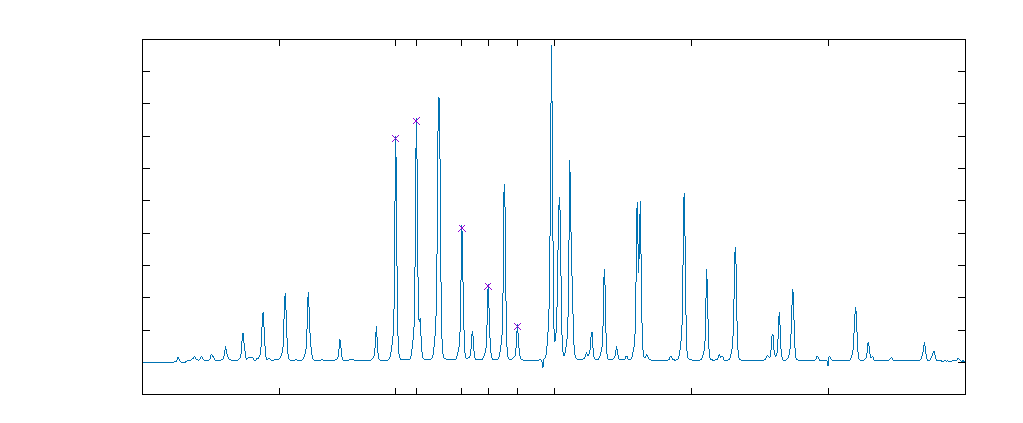
\includegraphics[width={475.20bp},height={187.20bp}]{OH7_data}}%
    \gplfronttext
  \end{picture}%
\endgroup

    \vspace{40pt}
    \captionsetup{type=graph}
    \caption{Naměřená spektrální závislost radikálů OH. Graf je korektovaný podle známých vlnových délek spektrálních čar a šumu pozadí.}
\end{figure}

\begin{table}[htpb]
    \vspace{-20pt}
    \begin{minipage}[t]{.5\linewidth}
Z tabulky 2 sestrojím graf pyrometrické přímky podle vztahu (4) a ze sklonu $ a = -\frac{B_{v'} hc}{kT} $  zjistím rotační teplotu plazmatu. 


\begin{align*}
    a &= -0.089 \pm 0.003 \\
    h &= 6.62607015 \cdot 10^{-34} \text{ Js} \\
    c &= 299792458 \text{ ms}^{-1} \\
    k &= 1.380649 \cdot 10^{-23}  \text{ JK}^{-1} \\
    B_{v'} &= 1696 \text{ m}^{-1} \\
    T &= 273 \pm 10  \text{ K}\\
\end{align*}

    \end{minipage} 
    \hfill
    \begin{minipage}[t]{.5\linewidth}
        \centering

\begin{figure}[H]
    \vspace{-40pt}
    \centering
    % GNUPLOT: LaTeX picture with Postscript
\begingroup
  \makeatletter
  \providecommand\color[2][]{%
    \GenericError{(gnuplot) \space\space\space\@spaces}{%
      Package color not loaded in conjunction with
      terminal option `colourtext'%
    }{See the gnuplot documentation for explanation.%
    }{Either use 'blacktext' in gnuplot or load the package
      color.sty in LaTeX.}%
    \renewcommand\color[2][]{}%
  }%
  \providecommand\includegraphics[2][]{%
    \GenericError{(gnuplot) \space\space\space\@spaces}{%
      Package graphicx or graphics not loaded%
    }{See the gnuplot documentation for explanation.%
    }{The gnuplot epslatex terminal needs graphicx.sty or graphics.sty.}%
    \renewcommand\includegraphics[2][]{}%
  }%
  \providecommand\rotatebox[2]{#2}%
  \@ifundefined{ifGPcolor}{%
    \newif\ifGPcolor
    \GPcolorfalse
  }{}%
  \@ifundefined{ifGPblacktext}{%
    \newif\ifGPblacktext
    \GPblacktexttrue
  }{}%
  % define a \g@addto@macro without @ in the name:
  \let\gplgaddtomacro\g@addto@macro
  % define empty templates for all commands taking text:
  \gdef\gplbacktext{}%
  \gdef\gplfronttext{}%
  \makeatother
  \ifGPblacktext
    % no textcolor at all
    \def\colorrgb#1{}%
    \def\colorgray#1{}%
  \else
    % gray or color?
    \ifGPcolor
      \def\colorrgb#1{\color[rgb]{#1}}%
      \def\colorgray#1{\color[gray]{#1}}%
      \expandafter\def\csname LTw\endcsname{\color{white}}%
      \expandafter\def\csname LTb\endcsname{\color{black}}%
      \expandafter\def\csname LTa\endcsname{\color{black}}%
      \expandafter\def\csname LT0\endcsname{\color[rgb]{1,0,0}}%
      \expandafter\def\csname LT1\endcsname{\color[rgb]{0,1,0}}%
      \expandafter\def\csname LT2\endcsname{\color[rgb]{0,0,1}}%
      \expandafter\def\csname LT3\endcsname{\color[rgb]{1,0,1}}%
      \expandafter\def\csname LT4\endcsname{\color[rgb]{0,1,1}}%
      \expandafter\def\csname LT5\endcsname{\color[rgb]{1,1,0}}%
      \expandafter\def\csname LT6\endcsname{\color[rgb]{0,0,0}}%
      \expandafter\def\csname LT7\endcsname{\color[rgb]{1,0.3,0}}%
      \expandafter\def\csname LT8\endcsname{\color[rgb]{0.5,0.5,0.5}}%
    \else
      % gray
      \def\colorrgb#1{\color{black}}%
      \def\colorgray#1{\color[gray]{#1}}%
      \expandafter\def\csname LTw\endcsname{\color{white}}%
      \expandafter\def\csname LTb\endcsname{\color{black}}%
      \expandafter\def\csname LTa\endcsname{\color{black}}%
      \expandafter\def\csname LT0\endcsname{\color{black}}%
      \expandafter\def\csname LT1\endcsname{\color{black}}%
      \expandafter\def\csname LT2\endcsname{\color{black}}%
      \expandafter\def\csname LT3\endcsname{\color{black}}%
      \expandafter\def\csname LT4\endcsname{\color{black}}%
      \expandafter\def\csname LT5\endcsname{\color{black}}%
      \expandafter\def\csname LT6\endcsname{\color{black}}%
      \expandafter\def\csname LT7\endcsname{\color{black}}%
      \expandafter\def\csname LT8\endcsname{\color{black}}%
    \fi
  \fi
    \setlength{\unitlength}{0.0500bp}%
    \ifx\gptboxheight\undefined%
      \newlength{\gptboxheight}%
      \newlength{\gptboxwidth}%
      \newsavebox{\gptboxtext}%
    \fi%
    \setlength{\fboxrule}{0.5pt}%
    \setlength{\fboxsep}{1pt}%
    \definecolor{tbcol}{rgb}{1,1,1}%
\begin{picture}(4320.00,2160.00)%
    \gplgaddtomacro\gplbacktext{%
      \csname LTb\endcsname%%
      \put(946,64){\makebox(0,0)[r]{\strut{}$26$}}%
      \put(946,272){\makebox(0,0)[r]{\strut{}$26.5$}}%
      \put(946,481){\makebox(0,0)[r]{\strut{}$27$}}%
      \put(946,689){\makebox(0,0)[r]{\strut{}$27.5$}}%
      \put(946,897){\makebox(0,0)[r]{\strut{}$28$}}%
      \put(946,1106){\makebox(0,0)[r]{\strut{}$28.5$}}%
      \put(946,1314){\makebox(0,0)[r]{\strut{}$29$}}%
      \put(946,1522){\makebox(0,0)[r]{\strut{}$29.5$}}%
      \put(946,1731){\makebox(0,0)[r]{\strut{}$30$}}%
      \put(946,1939){\makebox(0,0)[r]{\strut{}$30.5$}}%
      \put(1078,-156){\makebox(0,0){\strut{}$0$}}%
      \put(1394,-156){\makebox(0,0){\strut{}$5$}}%
      \put(1710,-156){\makebox(0,0){\strut{}$10$}}%
      \put(2026,-156){\makebox(0,0){\strut{}$15$}}%
      \put(2342,-156){\makebox(0,0){\strut{}$20$}}%
      \put(2659,-156){\makebox(0,0){\strut{}$25$}}%
      \put(2975,-156){\makebox(0,0){\strut{}$30$}}%
      \put(3291,-156){\makebox(0,0){\strut{}$35$}}%
      \put(3607,-156){\makebox(0,0){\strut{}$40$}}%
      \put(3923,-156){\makebox(0,0){\strut{}$45$}}%
    }%
    \gplgaddtomacro\gplfronttext{%
      \csname LTb\endcsname%%
      \put(209,1001){\rotatebox{-270}{\makebox(0,0){\strut{}$  \ln \frac{I \lambda^4 }{S} $}}}%
      \put(2500,-486){\makebox(0,0){\strut{}$ N' (N' + 1)$ }}%
      \csname LTb\endcsname%%
      \put(2936,1766){\makebox(0,0)[r]{\strut{}$ ax + b $}}%
    }%
    \gplbacktext
    \put(0,0){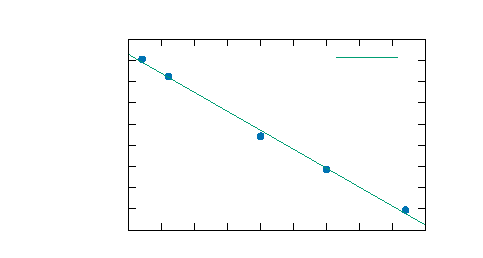
\includegraphics[width={216.00bp},height={108.00bp}]{intenzity}}%
    \gplfronttext
  \end{picture}%
\endgroup

    \captionsetup{type=graph}
    \caption{Pyrometrická přímka radikálů OH}
\end{figure}


    \end{minipage} 
\end{table}

\begin{table}[htpb]
    \vspace{-30pt}
    \centering
    \begin{tabular}{c c c c c}
        $ N' $  & $ J' $  & $ S_{J'J''} $ & $ \lambda_{nm} $ & $ I $  (a.u.)   \\\hline
        1 & 1/2 & 0.563 & 307.844 & 6.90 \\
        2 & 5/2 & 1.065 & 307.995 & 8.65 \\
        4 & 9/2 & 2.100 & 308.328 & 4.17 \\
        5 & 11/2 & 2.640 & 308.520 & 2.37 \\
        6 & 13/2 & 3.160 & 308.734 & 1.09 \\
    \end{tabular}
    \caption{Parametry rotačních spektrálních čar}
\end{table}

\newpage

\section{Závěr}

Pomocí programu Span 1.7 jsem zjistil intenzitu vybraných spektrálních čar par železa a z pyrometrické přímky určil teplotu plazmatu na $ T = 6000 \pm 500 $ K. Program zároveň umožňuje vyhodnotit teplotu automaticky, odkud mám hodnotu $ T = 6552 $ K. Rozdíl výsledků je pravděpodobně způsobený sofistikovanějším postupem, použitým v programu. 

Při vyhodnocování radikálů OH jsem použil jen 5 čar, ale zato vyšla velmi dobrá přímka a výsledná teplota $ T = 273 \pm 10 $ K má menší relativní nejistotu. Program znovu vyhodnotil teplotu o něco výš na $ T = 312 $, pravděpodobně ze stejného důvodu.

\begin{thebibliography}{0}
\bibitem{tabulky} Návod k úloze ~\url{https://is.muni.cz/auth/el/sci/jaro2025/F4210/um/fp3-7_spektra.pdf}.   
\end{thebibliography}

\end{document}
